%
% system_overview.tex
%
% Copyright (C) 2019 by SpaceLab.
%
% OBDH 2.0 Documentation
%
% This work is licensed under the Creative Commons Attribution-ShareAlike 4.0
% International License. To view a copy of this license,
% visit http://creativecommons.org/licenses/by-sa/4.0/.
%

%
% \brief System Overview chapter.
%
% \author Gabriel Mariano Marcelino <gabriel.mm8@gmail.com>
%
% \institution Universidade Federal de Santa Catarina (UFSC)
%
% \version 0.1.0
%
% \date 23/11/2019
%

\chapter{System Overview} \label{ch:system-overview}

\section{Block Diagram}

\begin{figure}[!ht]
    \begin{center}
        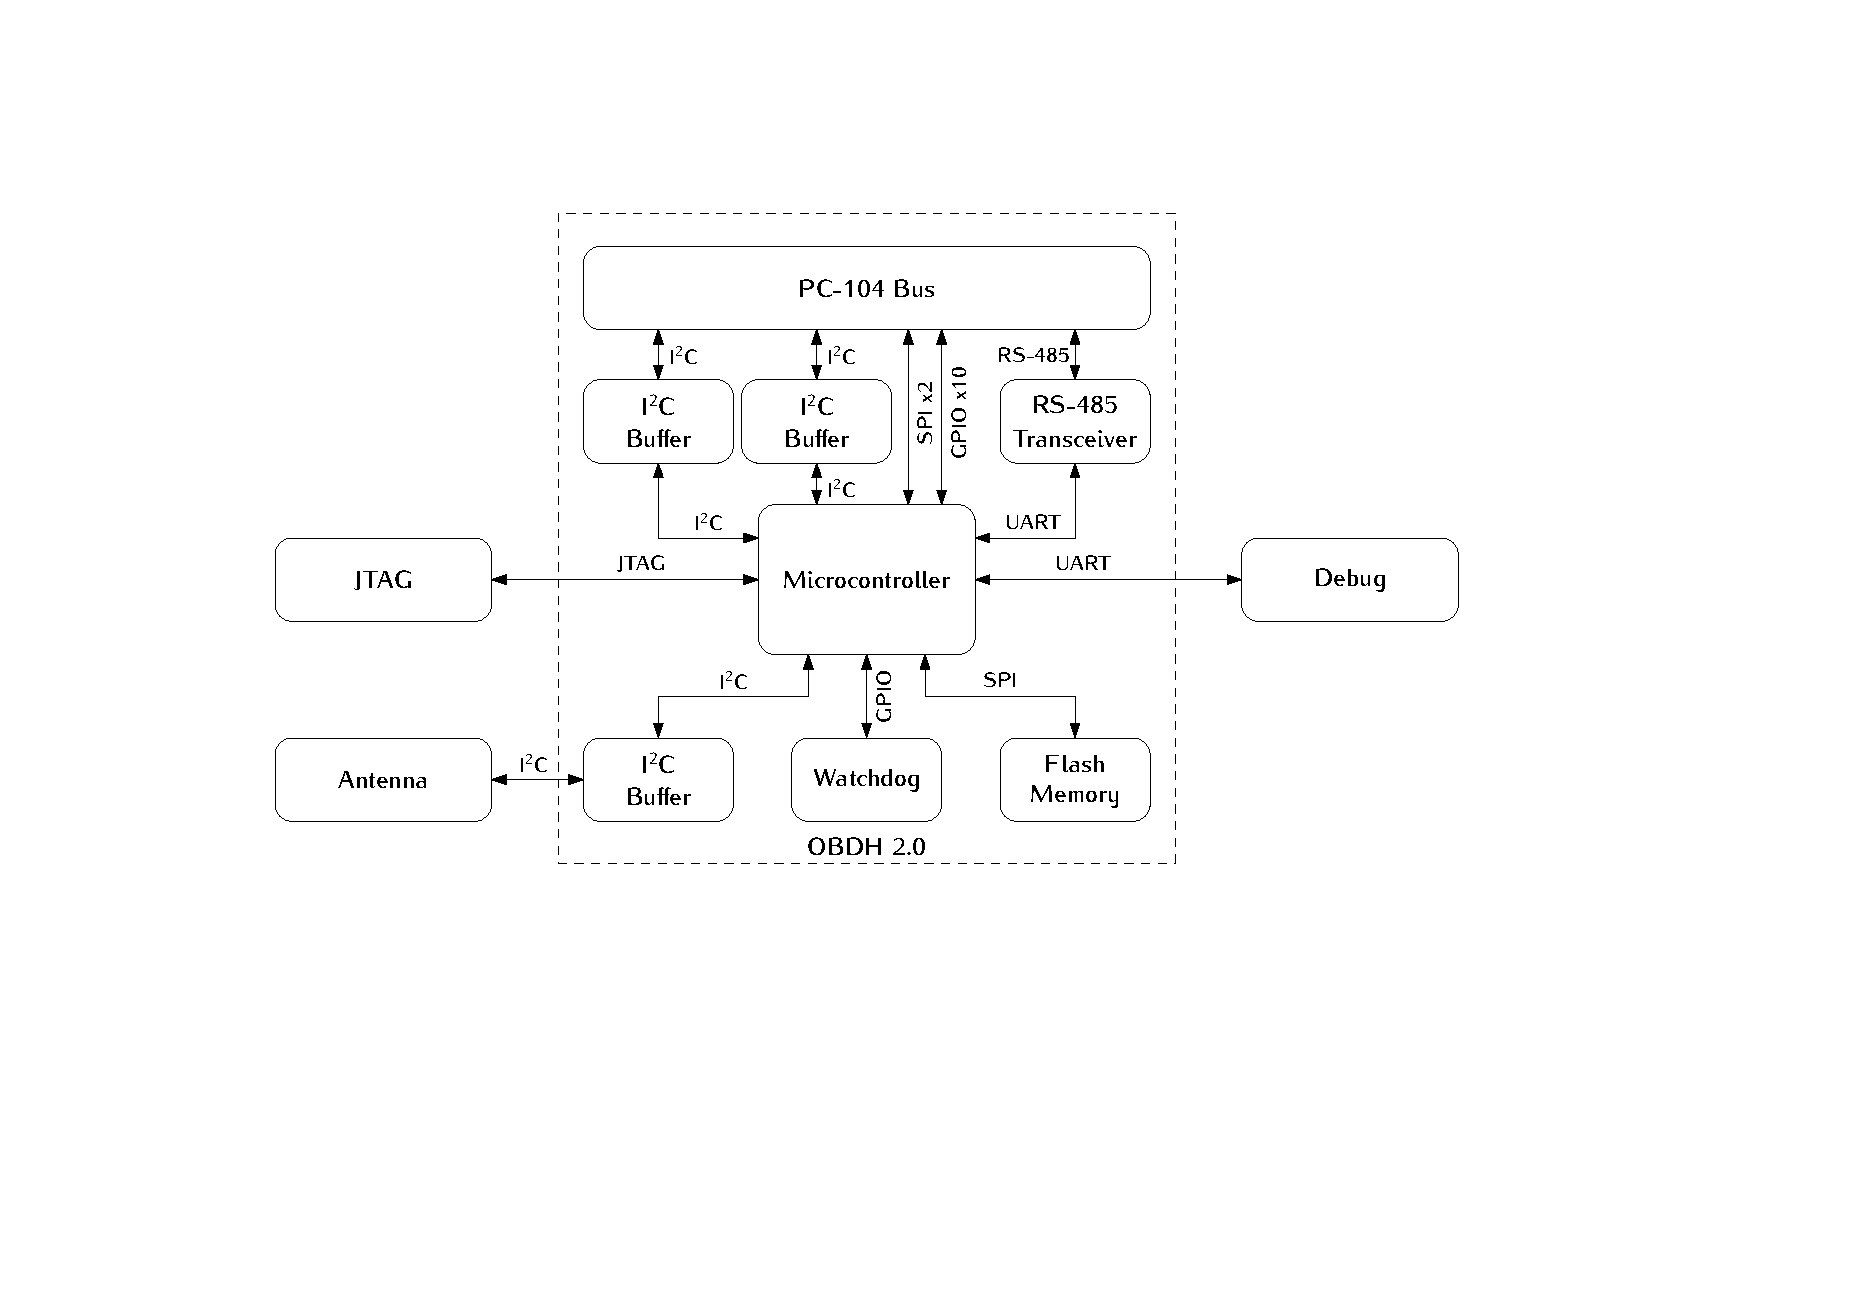
\includegraphics[width=\textwidth]{figures/block_diagram.pdf}
        \label{fig:block-diagram}
        \caption{OBDH 2.0 Block diagram.}
    \end{center}
\end{figure}

\section{System Layers}

\begin{figure}[!ht]
    \begin{center}
        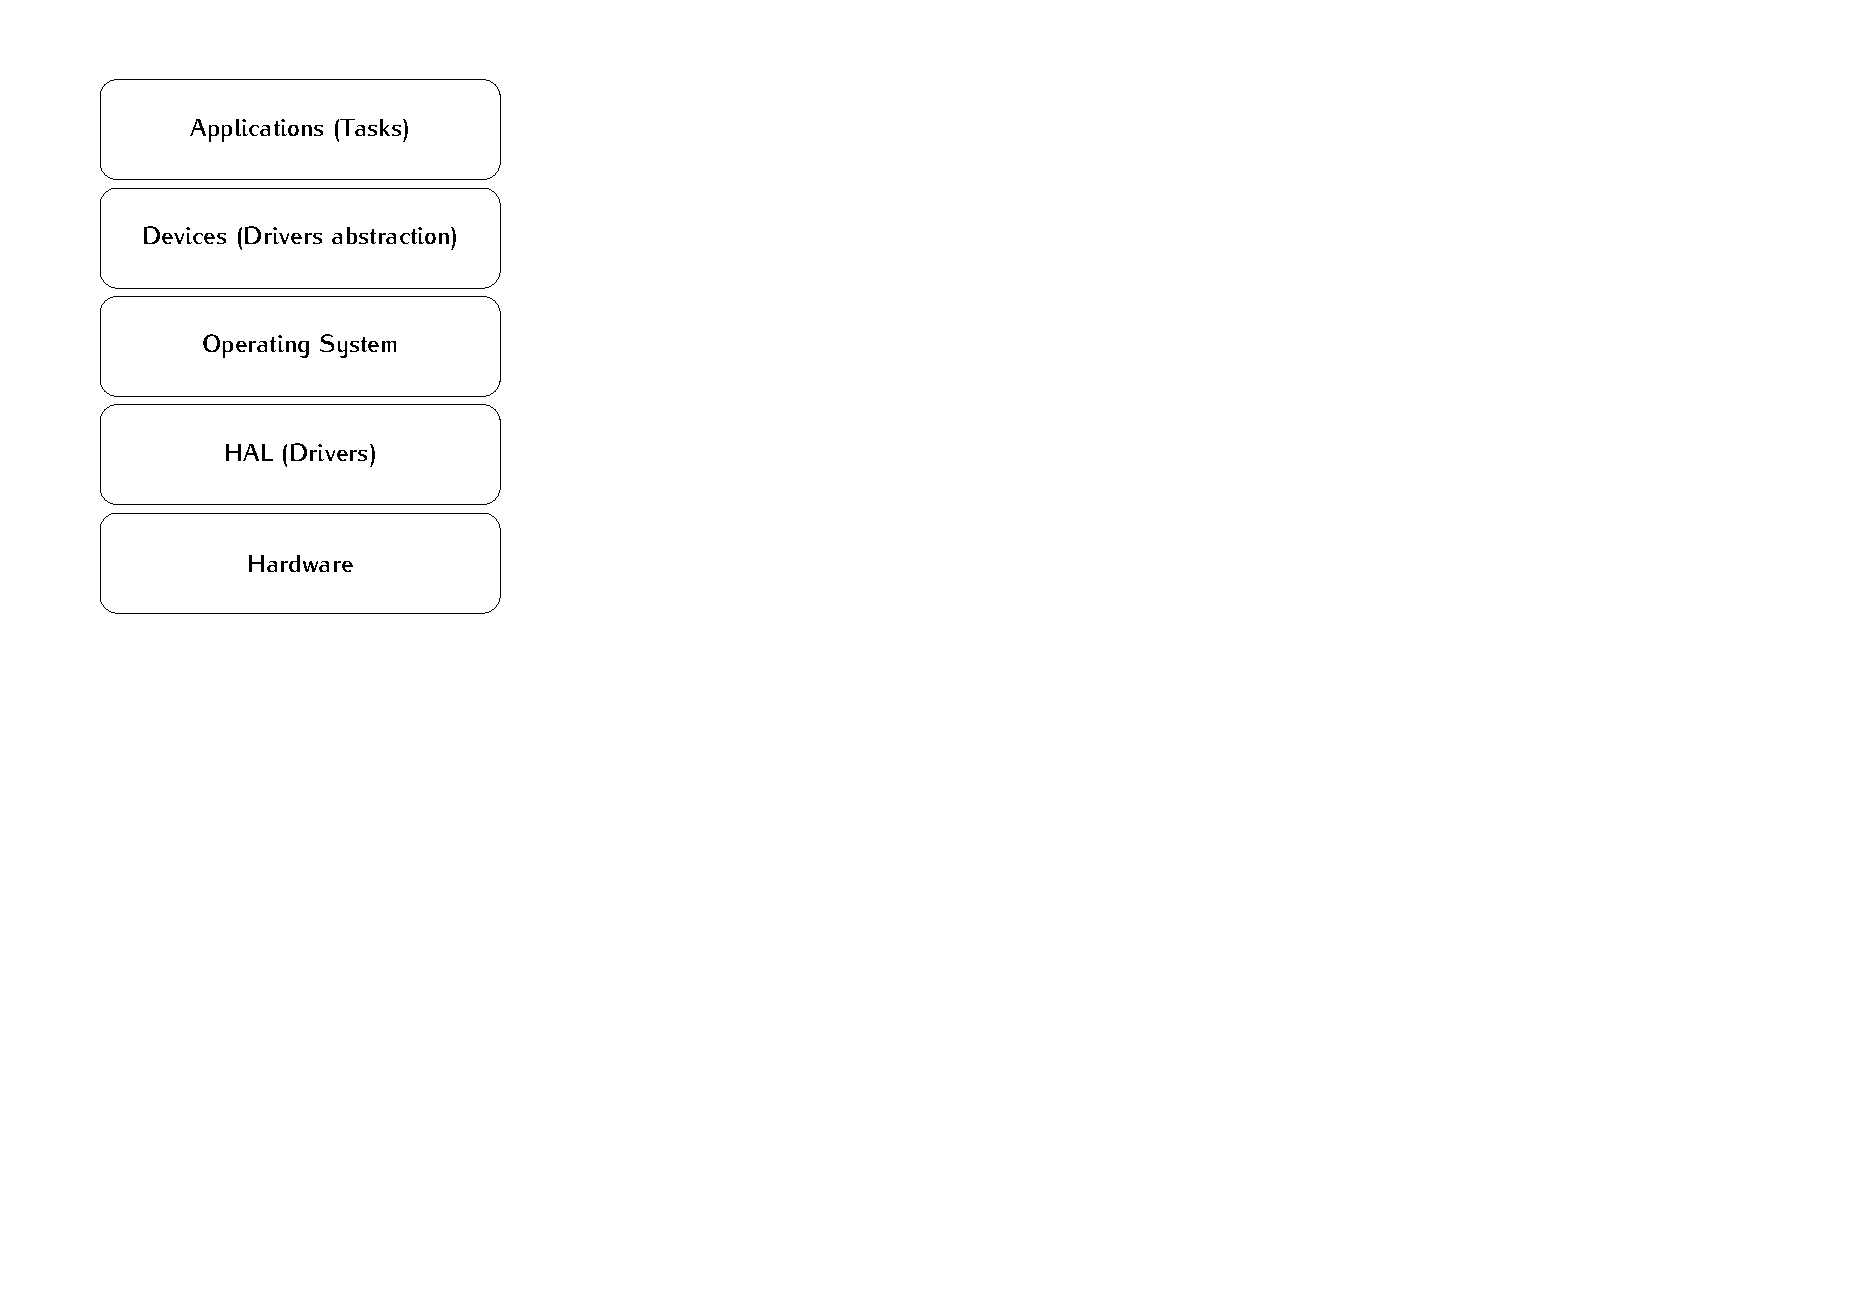
\includegraphics[width=0.4\textwidth]{figures/system_layers.pdf}
        \label{fig:system-layers}
        \caption{System layers.}
    \end{center}
\end{figure}

\section{Operation}

\subsection{Status LEDs}

On the development version of the board, there are eight LEDs that indicates some behaviours of the systems. This set of LEDs can be seen on \autoref{fig:status-leds}.

\begin{figure}[!ht]
    \begin{center}
        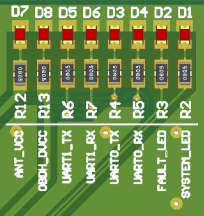
\includegraphics[width=0.3\textwidth]{figures/status_leds.png}
        \label{fig:status-leds}
        \caption{Available status LEDs.}
    \end{center}
\end{figure}

A description of each of these LEDs are available below:

\begin{itemize}
    \item \textbf{D1 - System LED}: Heartbeat of the system. Blinks at a frequency of 1 Hz when the system is running properly.
    \item \textbf{D2 - Fault LED}: Indicates a critical fault in the system.
    \item \textbf{D3 - UART0 TX}: Blinks when data is being transmitted over the UART0 port.
    \item \textbf{D4 - UART0 RX}: Blinks when data is being received over the UART0 port.
    \item \textbf{D5 - UART1 TX}: Blinks when data is being transmitted over that UART1 port.
    \item \textbf{D6 - UART1 RX}: Blinks when data is being received over the UART1 port.
    \item \textbf{D7 - Antenna VCC}: Indicates that the antenna module board is being power sourced.
    \item \textbf{D8 - OBDH VCC}: Indicates that the OBDH board is being power sourced.
\end{itemize}

These LEDs are not mounted in the flight version of the module.
